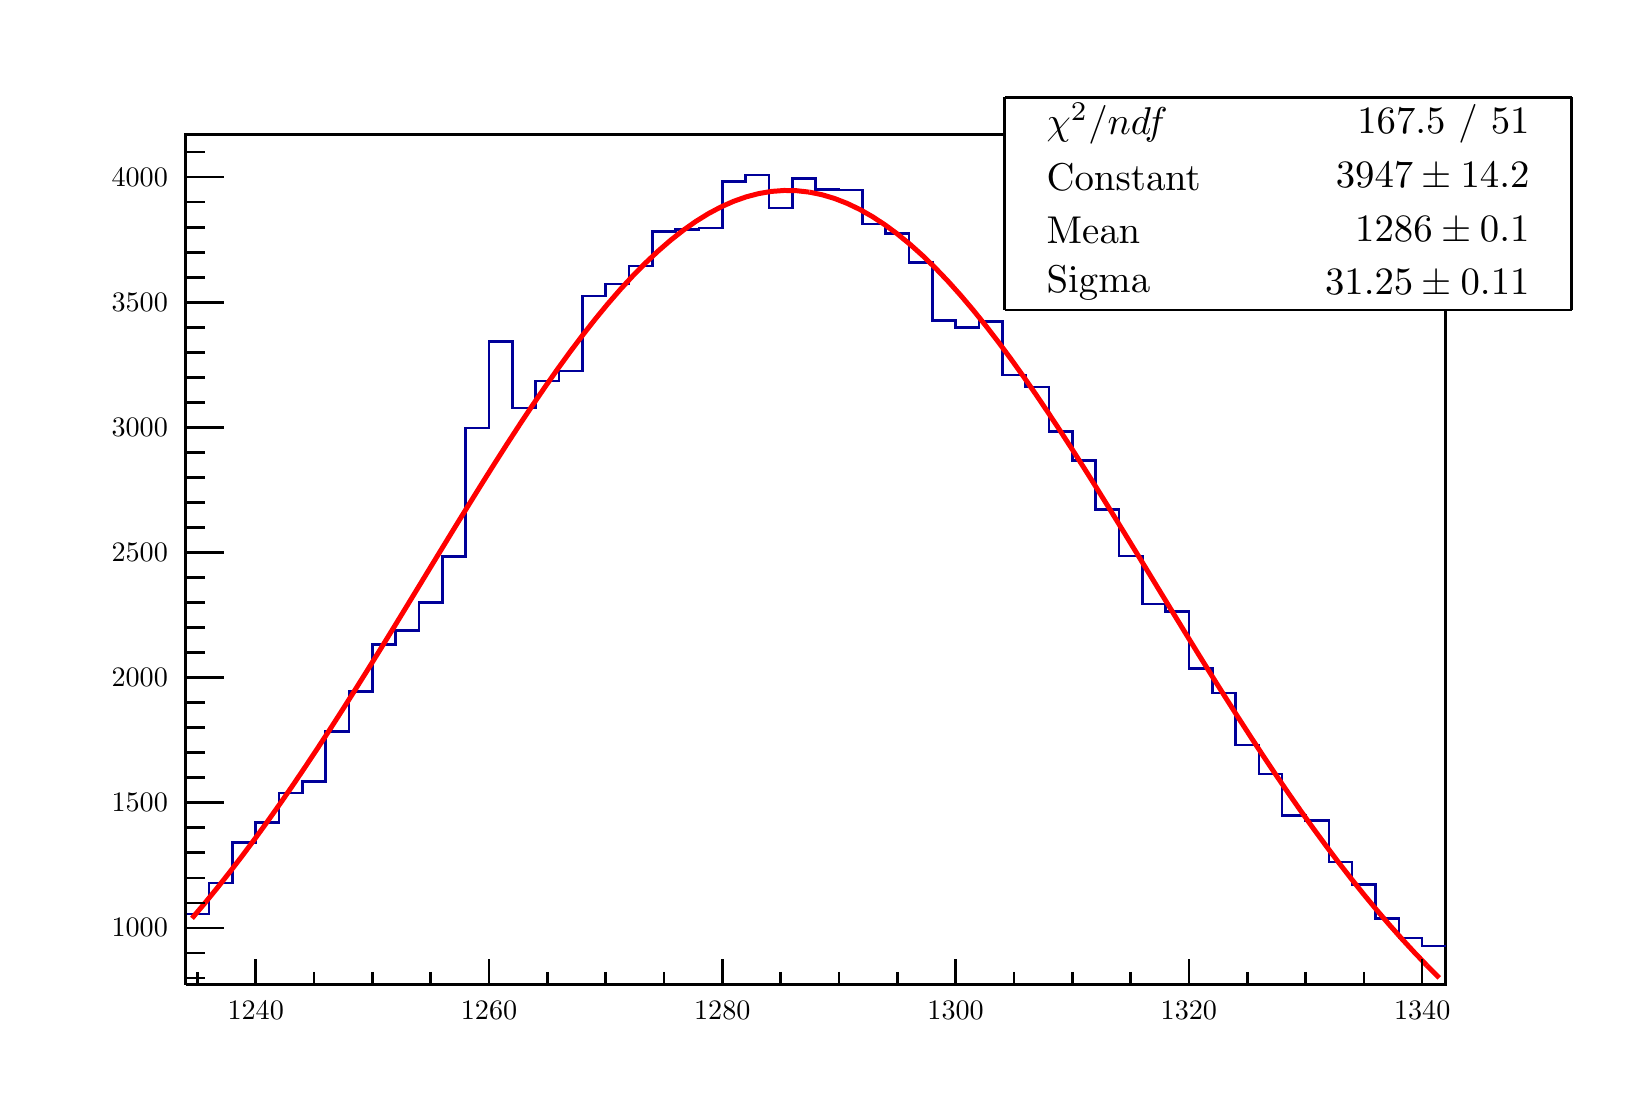
\begin{tikzpicture}
\pgfdeclareplotmark{cross} {
\pgfpathmoveto{\pgfpoint{-0.3\pgfplotmarksize}{\pgfplotmarksize}}
\pgfpathlineto{\pgfpoint{+0.3\pgfplotmarksize}{\pgfplotmarksize}}
\pgfpathlineto{\pgfpoint{+0.3\pgfplotmarksize}{0.3\pgfplotmarksize}}
\pgfpathlineto{\pgfpoint{+1\pgfplotmarksize}{0.3\pgfplotmarksize}}
\pgfpathlineto{\pgfpoint{+1\pgfplotmarksize}{-0.3\pgfplotmarksize}}
\pgfpathlineto{\pgfpoint{+0.3\pgfplotmarksize}{-0.3\pgfplotmarksize}}
\pgfpathlineto{\pgfpoint{+0.3\pgfplotmarksize}{-1.\pgfplotmarksize}}
\pgfpathlineto{\pgfpoint{-0.3\pgfplotmarksize}{-1.\pgfplotmarksize}}
\pgfpathlineto{\pgfpoint{-0.3\pgfplotmarksize}{-0.3\pgfplotmarksize}}
\pgfpathlineto{\pgfpoint{-1.\pgfplotmarksize}{-0.3\pgfplotmarksize}}
\pgfpathlineto{\pgfpoint{-1.\pgfplotmarksize}{0.3\pgfplotmarksize}}
\pgfpathlineto{\pgfpoint{-0.3\pgfplotmarksize}{0.3\pgfplotmarksize}}
\pgfpathclose
\pgfusepathqstroke
}
\pgfdeclareplotmark{cross*} {
\pgfpathmoveto{\pgfpoint{-0.3\pgfplotmarksize}{\pgfplotmarksize}}
\pgfpathlineto{\pgfpoint{+0.3\pgfplotmarksize}{\pgfplotmarksize}}
\pgfpathlineto{\pgfpoint{+0.3\pgfplotmarksize}{0.3\pgfplotmarksize}}
\pgfpathlineto{\pgfpoint{+1\pgfplotmarksize}{0.3\pgfplotmarksize}}
\pgfpathlineto{\pgfpoint{+1\pgfplotmarksize}{-0.3\pgfplotmarksize}}
\pgfpathlineto{\pgfpoint{+0.3\pgfplotmarksize}{-0.3\pgfplotmarksize}}
\pgfpathlineto{\pgfpoint{+0.3\pgfplotmarksize}{-1.\pgfplotmarksize}}
\pgfpathlineto{\pgfpoint{-0.3\pgfplotmarksize}{-1.\pgfplotmarksize}}
\pgfpathlineto{\pgfpoint{-0.3\pgfplotmarksize}{-0.3\pgfplotmarksize}}
\pgfpathlineto{\pgfpoint{-1.\pgfplotmarksize}{-0.3\pgfplotmarksize}}
\pgfpathlineto{\pgfpoint{-1.\pgfplotmarksize}{0.3\pgfplotmarksize}}
\pgfpathlineto{\pgfpoint{-0.3\pgfplotmarksize}{0.3\pgfplotmarksize}}
\pgfpathclose
\pgfusepathqfillstroke
}
\pgfdeclareplotmark{newstar} {
\pgfpathmoveto{\pgfqpoint{0pt}{\pgfplotmarksize}}
\pgfpathlineto{\pgfqpointpolar{44}{0.5\pgfplotmarksize}}
\pgfpathlineto{\pgfqpointpolar{18}{\pgfplotmarksize}}
\pgfpathlineto{\pgfqpointpolar{-20}{0.5\pgfplotmarksize}}
\pgfpathlineto{\pgfqpointpolar{-54}{\pgfplotmarksize}}
\pgfpathlineto{\pgfqpointpolar{-90}{0.5\pgfplotmarksize}}
\pgfpathlineto{\pgfqpointpolar{234}{\pgfplotmarksize}}
\pgfpathlineto{\pgfqpointpolar{198}{0.5\pgfplotmarksize}}
\pgfpathlineto{\pgfqpointpolar{162}{\pgfplotmarksize}}
\pgfpathlineto{\pgfqpointpolar{134}{0.5\pgfplotmarksize}}
\pgfpathclose
\pgfusepathqstroke
}
\pgfdeclareplotmark{newstar*} {
\pgfpathmoveto{\pgfqpoint{0pt}{\pgfplotmarksize}}
\pgfpathlineto{\pgfqpointpolar{44}{0.5\pgfplotmarksize}}
\pgfpathlineto{\pgfqpointpolar{18}{\pgfplotmarksize}}
\pgfpathlineto{\pgfqpointpolar{-20}{0.5\pgfplotmarksize}}
\pgfpathlineto{\pgfqpointpolar{-54}{\pgfplotmarksize}}
\pgfpathlineto{\pgfqpointpolar{-90}{0.5\pgfplotmarksize}}
\pgfpathlineto{\pgfqpointpolar{234}{\pgfplotmarksize}}
\pgfpathlineto{\pgfqpointpolar{198}{0.5\pgfplotmarksize}}
\pgfpathlineto{\pgfqpointpolar{162}{\pgfplotmarksize}}
\pgfpathlineto{\pgfqpointpolar{134}{0.5\pgfplotmarksize}}
\pgfpathclose
\pgfusepathqfillstroke
}
\definecolor{c}{rgb}{1,1,1};
\draw [color=c, fill=c] (0,0) rectangle (20,13.4957);
\draw [color=c, fill=c] (2,1.34957) rectangle (18,12.1461);
\definecolor{c}{rgb}{0,0,0};
\draw [c,line width=0.9] (2,1.34957) -- (2,12.1461) -- (18,12.1461) -- (18,1.34957) -- (2,1.34957);
\definecolor{c}{rgb}{1,1,1};
\draw [color=c, fill=c] (2,1.34957) rectangle (18,12.1461);
\definecolor{c}{rgb}{0,0,0};
\draw [c,line width=0.9] (2,1.34957) -- (2,12.1461) -- (18,12.1461) -- (18,1.34957) -- (2,1.34957);
\definecolor{c}{rgb}{0,0,0.6};
\draw [c,line width=0.9] (2,2.24592) -- (2.2963,2.24592) -- (2.2963,2.63992) -- (2.59259,2.63992) -- (2.59259,3.15466) -- (2.88889,3.15466) -- (2.88889,3.40568) -- (3.18519,3.40568) -- (3.18519,3.78061) -- (3.48148,3.78061) -- (3.48148,3.92995) --
 (3.77778,3.92995) -- (3.77778,4.56226) -- (4.07407,4.56226) -- (4.07407,5.07382) -- (4.37037,5.07382) -- (4.37037,5.67118) -- (4.66667,5.67118) -- (4.66667,5.84593) -- (4.96296,5.84593) -- (4.96296,6.20498) -- (5.25926,6.20498) -- (5.25926,6.78963)
 -- (5.55556,6.78963) -- (5.55556,8.41964) -- (5.85185,8.41964) -- (5.85185,9.51585) -- (6.14815,9.51585) -- (6.14815,8.67383) -- (6.44444,8.67383) -- (6.44444,9.01382) -- (6.74074,9.01382) -- (6.74074,9.14409) -- (7.03704,9.14409) --
 (7.03704,10.0941) -- (7.33333,10.0941) -- (7.33333,10.2498) -- (7.62963,10.2498) -- (7.62963,10.4754) -- (7.92593,10.4754) -- (7.92593,10.9171) -- (8.22222,10.9171) -- (8.22222,10.9425) -- (8.51852,10.9425) -- (8.51852,10.9616) -- (8.81481,10.9616)
 -- (8.81481,11.5494) -- (9.11111,11.5494) -- (9.11111,11.632) -- (9.40741,11.632) -- (9.40741,11.2094) -- (9.7037,11.2094) -- (9.7037,11.5875) -- (10,11.5875) -- (10,11.4477) -- (10.2963,11.4477) -- (10.2963,11.4414) -- (10.5926,11.4414) --
 (10.5926,11.0092) -- (10.8889,11.0092) -- (10.8889,10.8917) -- (11.1852,10.8917) -- (11.1852,10.5231) -- (11.4815,10.5231) -- (11.4815,9.78593) -- (11.7778,9.78593) -- (11.7778,9.69696) -- (12.0741,9.69696) -- (12.0741,9.77004) -- (12.3704,9.77004)
 -- (12.3704,9.09008) -- (12.6667,9.09008) -- (12.6667,8.93756) -- (12.963,8.93756) -- (12.963,8.37198) -- (13.2593,8.37198) -- (13.2593,8.0034) -- (13.5556,8.0034) -- (13.5556,7.3838) -- (13.8519,7.3838) -- (13.8519,6.7928) -- (14.1481,6.7928) --
 (14.1481,6.18274) -- (14.4444,6.18274) -- (14.4444,6.08742) -- (14.7407,6.08742) -- (14.7407,5.36297) -- (15.037,5.36297) -- (15.037,5.05158) -- (15.3333,5.05158) -- (15.3333,4.39068) -- (15.6296,4.39068) -- (15.6296,4.0221) -- (15.9259,4.0221) --
 (15.9259,3.49782) -- (16.2222,3.49782) -- (16.2222,3.4311) -- (16.5185,3.4311) -- (16.5185,2.90365) -- (16.8148,2.90365) -- (16.8148,2.62085) -- (17.1111,2.62085) -- (17.1111,2.18873) -- (17.4074,2.18873) -- (17.4074,1.94089) -- (17.7037,1.94089) --
 (17.7037,1.83921) -- (18,1.83921);
\definecolor{c}{rgb}{1,1,1};
\draw [color=c, fill=c] (12.4,9.91934) rectangle (19.6,12.6185);
\definecolor{c}{rgb}{0,0,0};
\draw [c,line width=0.9] (12.4,9.91934) -- (19.6,9.91934);
\draw [c,line width=0.9] (19.6,9.91934) -- (19.6,12.6185);
\draw [c,line width=0.9] (19.6,12.6185) -- (12.4,12.6185);
\draw [c,line width=0.9] (12.4,12.6185) -- (12.4,9.91934);
\draw [anchor= west] (12.76,12.2811) node[scale=1.40004, color=c, rotate=0]{$\chi^{2} / ndf $};
\draw [anchor= east] (19.24,12.2811) node[scale=1.40004, color=c, rotate=0]{ 167.5 / 51};
\draw [anchor= west] (12.76,11.6063) node[scale=1.40004, color=c, rotate=0]{Constant };
\draw [anchor= east] (19.24,11.6063) node[scale=1.40004, color=c, rotate=0]{$  3947 \pm 14.2$};
\draw [anchor= west] (12.76,10.9315) node[scale=1.40004, color=c, rotate=0]{Mean     };
\draw [anchor= east] (19.24,10.9315) node[scale=1.40004, color=c, rotate=0]{$  1286 \pm 0.1$};
\draw [anchor= west] (12.76,10.2567) node[scale=1.40004, color=c, rotate=0]{Sigma    };
\draw [anchor= east] (19.24,10.2567) node[scale=1.40004, color=c, rotate=0]{$ 31.25 \pm 0.11$};
\definecolor{c}{rgb}{1,0,0};
\draw [c,line width=1.8] (2.08,2.19136) -- (2.24,2.38092) -- (2.4,2.57696) -- (2.56,2.77939) -- (2.72,2.98805) -- (2.88,3.20276) -- (3.04,3.42332) -- (3.2,3.64949) -- (3.36,3.88099) -- (3.52,4.11752) -- (3.68,4.35873) -- (3.84,4.60426) -- (4,4.8537)
 -- (4.16,5.10661) -- (4.32,5.36252) -- (4.48,5.62093) -- (4.64,5.88132) -- (4.8,6.14312) -- (4.96,6.40575) -- (5.12,6.66861) -- (5.28,6.93106) -- (5.44,7.19245) -- (5.6,7.45212) -- (5.76,7.70938) -- (5.92,7.96353) -- (6.08,8.21387) -- (6.24,8.45969)
 -- (6.4,8.70027) -- (6.56,8.93491) -- (6.72,9.16289) -- (6.88,9.38351) -- (7.04,9.59608) -- (7.2,9.79992) -- (7.36,9.99438) -- (7.52,10.1788) -- (7.68,10.3526) -- (7.84,10.5152) -- (8,10.6661) -- (8.16,10.8047) -- (8.32,10.9305) -- (8.48,11.0431) --
 (8.64,11.1421) -- (8.8,11.2272) -- (8.96,11.2981) -- (9.12,11.3545) -- (9.28,11.3962) -- (9.44,11.4231) -- (9.6,11.4351) -- (9.76,11.432) -- (9.92,11.414);
\draw [c,line width=1.8] (9.92,11.414) -- (10.08,11.3812) -- (10.24,11.3335) -- (10.4,11.2712) -- (10.56,11.1946) -- (10.72,11.1038) -- (10.88,10.9992) -- (11.04,10.8812) -- (11.2,10.7502) -- (11.36,10.6066) -- (11.52,10.451) -- (11.68,10.2838) --
 (11.84,10.1056) -- (12,9.91705) -- (12.16,9.71872) -- (12.32,9.51128) -- (12.48,9.29538) -- (12.64,9.0717) -- (12.8,8.84095) -- (12.96,8.60383) -- (13.12,8.36105) -- (13.28,8.11332) -- (13.44,7.86135) -- (13.6,7.60586) -- (13.76,7.34755) --
 (13.92,7.0871) -- (14.08,6.8252) -- (14.24,6.56251) -- (14.4,6.29967) -- (14.56,6.0373) -- (14.72,5.776) -- (14.88,5.51635) -- (15.04,5.25888) -- (15.2,5.00413) -- (15.36,4.75256) -- (15.52,4.50465) -- (15.68,4.26082) -- (15.84,4.02145) --
 (16,3.78692) -- (16.16,3.55753) -- (16.32,3.3336) -- (16.48,3.11537) -- (16.64,2.90308) -- (16.8,2.69691) -- (16.96,2.49705) -- (17.12,2.30361) -- (17.28,2.1167) -- (17.44,1.93641) -- (17.6,1.76277) -- (17.76,1.59581);
\draw [c,line width=1.8] (17.76,1.59581) -- (17.92,1.43553);
\definecolor{c}{rgb}{0,0,0};
\draw [c,line width=0.9] (2,1.34957) -- (18,1.34957);
\draw [c,line width=0.9] (2.88889,1.67347) -- (2.88889,1.34957);
\draw [c,line width=0.9] (3.62963,1.51152) -- (3.62963,1.34957);
\draw [c,line width=0.9] (4.37037,1.51152) -- (4.37037,1.34957);
\draw [c,line width=0.9] (5.11111,1.51152) -- (5.11111,1.34957);
\draw [c,line width=0.9] (5.85185,1.67347) -- (5.85185,1.34957);
\draw [c,line width=0.9] (6.59259,1.51152) -- (6.59259,1.34957);
\draw [c,line width=0.9] (7.33333,1.51152) -- (7.33333,1.34957);
\draw [c,line width=0.9] (8.07407,1.51152) -- (8.07407,1.34957);
\draw [c,line width=0.9] (8.81481,1.67347) -- (8.81481,1.34957);
\draw [c,line width=0.9] (9.55556,1.51152) -- (9.55556,1.34957);
\draw [c,line width=0.9] (10.2963,1.51152) -- (10.2963,1.34957);
\draw [c,line width=0.9] (11.037,1.51152) -- (11.037,1.34957);
\draw [c,line width=0.9] (11.7778,1.67347) -- (11.7778,1.34957);
\draw [c,line width=0.9] (12.5185,1.51152) -- (12.5185,1.34957);
\draw [c,line width=0.9] (13.2593,1.51152) -- (13.2593,1.34957);
\draw [c,line width=0.9] (14,1.51152) -- (14,1.34957);
\draw [c,line width=0.9] (14.7407,1.67347) -- (14.7407,1.34957);
\draw [c,line width=0.9] (15.4815,1.51152) -- (15.4815,1.34957);
\draw [c,line width=0.9] (16.2222,1.51152) -- (16.2222,1.34957);
\draw [c,line width=0.9] (16.963,1.51152) -- (16.963,1.34957);
\draw [c,line width=0.9] (17.7037,1.67347) -- (17.7037,1.34957);
\draw [c,line width=0.9] (2.88889,1.67347) -- (2.88889,1.34957);
\draw [c,line width=0.9] (2.14815,1.51152) -- (2.14815,1.34957);
\draw [c,line width=0.9] (17.7037,1.67347) -- (17.7037,1.34957);
\draw [anchor=base] (2.88889,0.904212) node[scale=1.01821, color=c, rotate=0]{1240};
\draw [anchor=base] (5.85185,0.904212) node[scale=1.01821, color=c, rotate=0]{1260};
\draw [anchor=base] (8.81481,0.904212) node[scale=1.01821, color=c, rotate=0]{1280};
\draw [anchor=base] (11.7778,0.904212) node[scale=1.01821, color=c, rotate=0]{1300};
\draw [anchor=base] (14.7407,0.904212) node[scale=1.01821, color=c, rotate=0]{1320};
\draw [anchor=base] (17.7037,0.904212) node[scale=1.01821, color=c, rotate=0]{1340};
\draw [c,line width=0.9] (2,1.34957) -- (2,12.1461);
\draw [c,line width=0.9] (2.48,2.07116) -- (2,2.07116);
\draw [c,line width=0.9] (2.24,2.3889) -- (2,2.3889);
\draw [c,line width=0.9] (2.24,2.70665) -- (2,2.70665);
\draw [c,line width=0.9] (2.24,3.02439) -- (2,3.02439);
\draw [c,line width=0.9] (2.24,3.34213) -- (2,3.34213);
\draw [c,line width=0.9] (2.48,3.65987) -- (2,3.65987);
\draw [c,line width=0.9] (2.24,3.97761) -- (2,3.97761);
\draw [c,line width=0.9] (2.24,4.29535) -- (2,4.29535);
\draw [c,line width=0.9] (2.24,4.6131) -- (2,4.6131);
\draw [c,line width=0.9] (2.24,4.93084) -- (2,4.93084);
\draw [c,line width=0.9] (2.48,5.24858) -- (2,5.24858);
\draw [c,line width=0.9] (2.24,5.56632) -- (2,5.56632);
\draw [c,line width=0.9] (2.24,5.88406) -- (2,5.88406);
\draw [c,line width=0.9] (2.24,6.2018) -- (2,6.2018);
\draw [c,line width=0.9] (2.24,6.51955) -- (2,6.51955);
\draw [c,line width=0.9] (2.48,6.83729) -- (2,6.83729);
\draw [c,line width=0.9] (2.24,7.15503) -- (2,7.15503);
\draw [c,line width=0.9] (2.24,7.47277) -- (2,7.47277);
\draw [c,line width=0.9] (2.24,7.79051) -- (2,7.79051);
\draw [c,line width=0.9] (2.24,8.10825) -- (2,8.10825);
\draw [c,line width=0.9] (2.48,8.426) -- (2,8.426);
\draw [c,line width=0.9] (2.24,8.74374) -- (2,8.74374);
\draw [c,line width=0.9] (2.24,9.06148) -- (2,9.06148);
\draw [c,line width=0.9] (2.24,9.37922) -- (2,9.37922);
\draw [c,line width=0.9] (2.24,9.69696) -- (2,9.69696);
\draw [c,line width=0.9] (2.48,10.0147) -- (2,10.0147);
\draw [c,line width=0.9] (2.24,10.3324) -- (2,10.3324);
\draw [c,line width=0.9] (2.24,10.6502) -- (2,10.6502);
\draw [c,line width=0.9] (2.24,10.9679) -- (2,10.9679);
\draw [c,line width=0.9] (2.24,11.2857) -- (2,11.2857);
\draw [c,line width=0.9] (2.48,11.6034) -- (2,11.6034);
\draw [c,line width=0.9] (2.48,2.07116) -- (2,2.07116);
\draw [c,line width=0.9] (2.24,1.75342) -- (2,1.75342);
\draw [c,line width=0.9] (2.24,1.43568) -- (2,1.43568);
\draw [c,line width=0.9] (2.48,11.6034) -- (2,11.6034);
\draw [c,line width=0.9] (2.24,11.9212) -- (2,11.9212);
\draw [anchor= east] (1.9,2.07116) node[scale=1.01821, color=c, rotate=0]{1000};
\draw [anchor= east] (1.9,3.65987) node[scale=1.01821, color=c, rotate=0]{1500};
\draw [anchor= east] (1.9,5.24858) node[scale=1.01821, color=c, rotate=0]{2000};
\draw [anchor= east] (1.9,6.83729) node[scale=1.01821, color=c, rotate=0]{2500};
\draw [anchor= east] (1.9,8.426) node[scale=1.01821, color=c, rotate=0]{3000};
\draw [anchor= east] (1.9,10.0147) node[scale=1.01821, color=c, rotate=0]{3500};
\draw [anchor= east] (1.9,11.6034) node[scale=1.01821, color=c, rotate=0]{4000};
\definecolor{c}{rgb}{1,1,1};
\draw [color=c, fill=c] (12.4,9.91934) rectangle (19.6,12.6185);
\definecolor{c}{rgb}{0,0,0};
\draw [c,line width=0.9] (12.4,9.91934) -- (19.6,9.91934);
\draw [c,line width=0.9] (19.6,9.91934) -- (19.6,12.6185);
\draw [c,line width=0.9] (19.6,12.6185) -- (12.4,12.6185);
\draw [c,line width=0.9] (12.4,12.6185) -- (12.4,9.91934);
\draw [anchor= west] (12.76,12.2811) node[scale=1.40004, color=c, rotate=0]{$\chi^{2} / ndf $};
\draw [anchor= east] (19.24,12.2811) node[scale=1.40004, color=c, rotate=0]{ 167.5 / 51};
\draw [anchor= west] (12.76,11.6063) node[scale=1.40004, color=c, rotate=0]{Constant };
\draw [anchor= east] (19.24,11.6063) node[scale=1.40004, color=c, rotate=0]{$  3947 \pm 14.2$};
\draw [anchor= west] (12.76,10.9315) node[scale=1.40004, color=c, rotate=0]{Mean     };
\draw [anchor= east] (19.24,10.9315) node[scale=1.40004, color=c, rotate=0]{$  1286 \pm 0.1$};
\draw [anchor= west] (12.76,10.2567) node[scale=1.40004, color=c, rotate=0]{Sigma    };
\draw [anchor= east] (19.24,10.2567) node[scale=1.40004, color=c, rotate=0]{$ 31.25 \pm 0.11$};
\end{tikzpicture}
